% Options for packages loaded elsewhere
\PassOptionsToPackage{unicode}{hyperref}
\PassOptionsToPackage{hyphens}{url}
\PassOptionsToPackage{dvipsnames,svgnames*,x11names*}{xcolor}
%
\documentclass[
]{article}
\usepackage{lmodern}
\usepackage{amssymb,amsmath}
\usepackage{ifxetex,ifluatex}
\ifnum 0\ifxetex 1\fi\ifluatex 1\fi=0 % if pdftex
  \usepackage[T1]{fontenc}
  \usepackage[utf8]{inputenc}
  \usepackage{textcomp} % provide euro and other symbols
\else % if luatex or xetex
  \usepackage{unicode-math}
  \defaultfontfeatures{Scale=MatchLowercase}
  \defaultfontfeatures[\rmfamily]{Ligatures=TeX,Scale=1}
\fi
% Use upquote if available, for straight quotes in verbatim environments
\IfFileExists{upquote.sty}{\usepackage{upquote}}{}
\IfFileExists{microtype.sty}{% use microtype if available
  \usepackage[]{microtype}
  \UseMicrotypeSet[protrusion]{basicmath} % disable protrusion for tt fonts
}{}
\makeatletter
\@ifundefined{KOMAClassName}{% if non-KOMA class
  \IfFileExists{parskip.sty}{%
    \usepackage{parskip}
  }{% else
    \setlength{\parindent}{0pt}
    \setlength{\parskip}{6pt plus 2pt minus 1pt}}
}{% if KOMA class
  \KOMAoptions{parskip=half}}
\makeatother
\usepackage{xcolor}
\IfFileExists{xurl.sty}{\usepackage{xurl}}{} % add URL line breaks if available
\IfFileExists{bookmark.sty}{\usepackage{bookmark}}{\usepackage{hyperref}}
\hypersetup{
  pdftitle={My Excellent Research},
  pdfauthor={Dan Ovando; Daniel Ovando},
  colorlinks=true,
  linkcolor=blue,
  filecolor=Maroon,
  citecolor=Blue,
  urlcolor=Blue,
  pdfcreator={LaTeX via pandoc}}
\urlstyle{same} % disable monospaced font for URLs
\usepackage[margin=1in]{geometry}
\usepackage{longtable,booktabs}
% Correct order of tables after \paragraph or \subparagraph
\usepackage{etoolbox}
\makeatletter
\patchcmd\longtable{\par}{\if@noskipsec\mbox{}\fi\par}{}{}
\makeatother
% Allow footnotes in longtable head/foot
\IfFileExists{footnotehyper.sty}{\usepackage{footnotehyper}}{\usepackage{footnote}}
\makesavenoteenv{longtable}
\usepackage{graphicx}
\makeatletter
\def\maxwidth{\ifdim\Gin@nat@width>\linewidth\linewidth\else\Gin@nat@width\fi}
\def\maxheight{\ifdim\Gin@nat@height>\textheight\textheight\else\Gin@nat@height\fi}
\makeatother
% Scale images if necessary, so that they will not overflow the page
% margins by default, and it is still possible to overwrite the defaults
% using explicit options in \includegraphics[width, height, ...]{}
\setkeys{Gin}{width=\maxwidth,height=\maxheight,keepaspectratio}
% Set default figure placement to htbp
\makeatletter
\def\fps@figure{htbp}
\makeatother
\setlength{\emergencystretch}{3em} % prevent overfull lines
\providecommand{\tightlist}{%
  \setlength{\itemsep}{0pt}\setlength{\parskip}{0pt}}
\setcounter{secnumdepth}{5}
\usepackage{setspace}\doublespacing
\usepackage{lineno}\linenumbers
\usepackage{booktabs}
\usepackage{longtable}
\usepackage{array}
\usepackage{multirow}
\usepackage{wrapfig}
\usepackage{float}
\usepackage{colortbl}
\usepackage{pdflscape}
\usepackage{tabu}
\usepackage{threeparttable}
\usepackage{threeparttablex}
\usepackage[normalem]{ulem}
\usepackage{makecell}
\usepackage{xcolor}

\title{My Excellent Research}
\author{Dan Ovando \and Daniel Ovando}
\date{2020-11-16}

\begin{document}
\maketitle

{
\hypersetup{linkcolor=}
\setcounter{tocdepth}{2}
\tableofcontents
}
\hypertarget{introduction}{%
\section{Introduction}\label{introduction}}

We found some cool stuff (Fig.\ref{fig:main-fig})

\begin{figure}
\centering
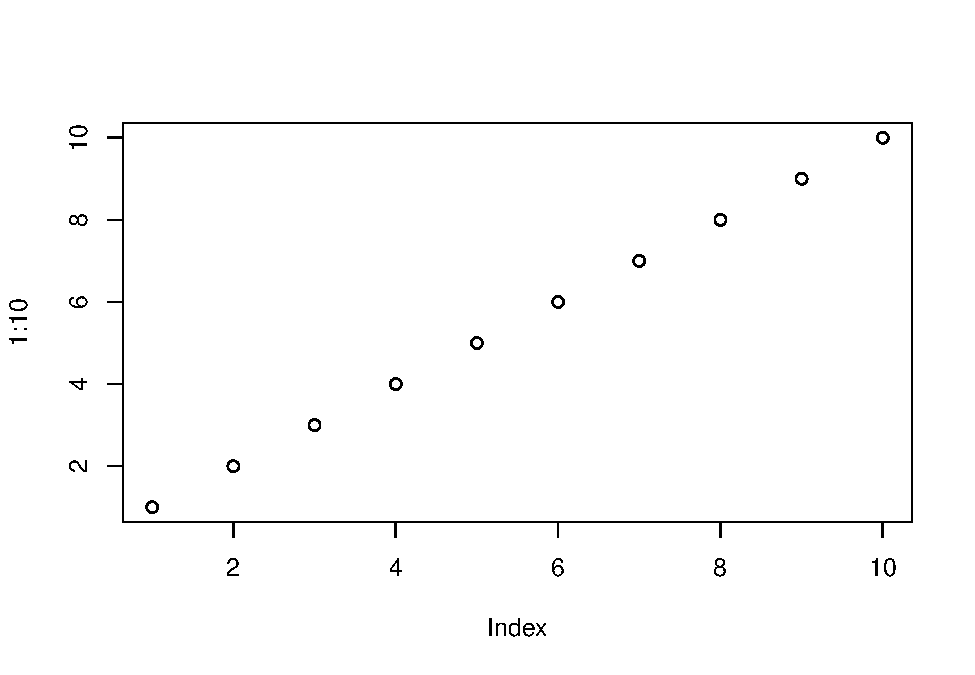
\includegraphics{my-pub_files/figure-latex/main-fig-1.pdf}
\caption{\label{fig:main-fig}Our Main Results}
\end{figure}

Here are some penguins (Table.\ref{tab:pen-tab})

\begin{longtable}[t]{llrrrrlr}
\caption{\label{tab:pen-tab}Here are some penguins}\\
\toprule
species & island & bill\_length\_mm & bill\_depth\_mm & flipper\_length\_mm & body\_mass\_g & sex & year\\
\midrule
\cellcolor{gray!6}{Adelie} & \cellcolor{gray!6}{Torgersen} & \cellcolor{gray!6}{39.1} & \cellcolor{gray!6}{18.7} & \cellcolor{gray!6}{181} & \cellcolor{gray!6}{3750} & \cellcolor{gray!6}{male} & \cellcolor{gray!6}{2007}\\
Adelie & Torgersen & 39.5 & 17.4 & 186 & 3800 & female & 2007\\
\cellcolor{gray!6}{Adelie} & \cellcolor{gray!6}{Torgersen} & \cellcolor{gray!6}{40.3} & \cellcolor{gray!6}{18.0} & \cellcolor{gray!6}{195} & \cellcolor{gray!6}{3250} & \cellcolor{gray!6}{female} & \cellcolor{gray!6}{2007}\\
Adelie & Torgersen & NA & NA & NA & NA & NA & 2007\\
\cellcolor{gray!6}{Adelie} & \cellcolor{gray!6}{Torgersen} & \cellcolor{gray!6}{36.7} & \cellcolor{gray!6}{19.3} & \cellcolor{gray!6}{193} & \cellcolor{gray!6}{3450} & \cellcolor{gray!6}{female} & \cellcolor{gray!6}{2007}\\
\addlinespace
Adelie & Torgersen & 39.3 & 20.6 & 190 & 3650 & male & 2007\\
\bottomrule
\end{longtable}

Here is a manual table, Tab.\ref{tab:simple-table}.

\newpage

This is a manual table (Table.\ref{tab:simple-table})

\begin{longtable}[]{@{}lll@{}}
\caption{\label{tab:simple-table} Caption for a Manual Table}\tabularnewline
\toprule
Thing 1 & Thing 2 & Col3\tabularnewline
\midrule
\endfirsthead
\toprule
Thing 1 & Thing 2 & Col3\tabularnewline
\midrule
\endhead
A & B & C\tabularnewline
D & E & F\tabularnewline
G & H & I\tabularnewline
\bottomrule
\end{longtable}

Here is a flipper model (Table.\ref{tab:flipper-model})

\begin{table}

\caption{\label{tab:flipper-model}My flipper model}
\centering
\begin{tabular}[t]{lc}
\toprule
  & Flipper Model\\
\midrule
(Intercept) & 209.707***\\
 & (0.862)\\
islandDream & -16.634***\\
 & (1.321)\\
islandTorgersen & -18.511***\\
 & (1.782)\\
\midrule
Num.Obs. & 342\\
R2 & 0.376\\
R2 Adj. & 0.372\\
AIC & 2624.4\\
BIC & 2639.7\\
Log.Lik. & -1308.197\\
F & 102.129\\
\bottomrule
\multicolumn{2}{l}{\textsuperscript{} * p < 0.1, ** p < 0.05, *** p <}\\
\multicolumn{2}{l}{0.01}\\
\end{tabular}
\end{table}

As you can see in Equation.\eqref{eq:binom}

\begin{equation} 
  f\left(k\right) = \binom{n}{k} p^k\left(1-p\right)^{n-k}
  \label{eq:binom}
\end{equation}

\newpage

\hypertarget{supplementary-materials}{%
\section{Supplementary Materials}\label{supplementary-materials}}

\renewcommand{\thefigure}{S\arabic{figure}}

\setcounter{figure}{0}

\renewcommand{\thetable}{S\arabic{table}}

\setcounter{table}{0}

\renewcommand{\theequation}{S\arabic{equation}}

\setcounter{equation}{0}

Here are our Supplementary materials\ldots{}

Here is another flipper model (Table.\ref{tab:si-flipper-model})

\begin{table}

\caption{\label{tab:si-flipper-model}My SI flipper model}
\centering
\begin{tabular}[t]{lc}
\toprule
  & SI Flipper Model\\
\midrule
(Intercept) & 188.795***\\
 & (0.999)\\
islandDream & 0.937\\
 & (1.336)\\
islandTorgersen & 2.401*\\
 & (1.364)\\
speciesChinstrap & 6.091***\\
 & (1.196)\\
speciesGentoo & 28.392***\\
 & (1.165)\\
\midrule
Num.Obs. & 342\\
R2 & 0.780\\
R2 Adj. & 0.778\\
AIC & 2271.4\\
BIC & 2294.4\\
Log.Lik. & -1129.679\\
F & 299.249\\
\bottomrule
\multicolumn{2}{l}{\textsuperscript{} * p < 0.1, ** p < 0.05, *** p <}\\
\multicolumn{2}{l}{0.01}\\
\end{tabular}
\end{table}

As you can see in Equation.\eqref{eq:binom2}

\begin{equation} 
  f\left(k\right) = \binom{n}{k} p^k\left(1-p\right)^{n-k}
  \label{eq:binom2}
\end{equation}

\newpage

\hypertarget{appendix}{%
\section{Appendix}\label{appendix}}

\renewcommand{\thefigure}{A\arabic{figure}}

\setcounter{figure}{0}

\renewcommand{\thetable}{A\arabic{table}}

\setcounter{table}{0}

\renewcommand{\theequation}{A\arabic{equation}}

\setcounter{equation}{0}

This is an appendix

As you can see in Equation.\eqref{eq:binom3}

\begin{equation} 
  f\left(k\right) = \binom{n}{k} p^k\left(1-p\right)^{n-k}
  \label{eq:binom3}
\end{equation}

\end{document}
